\chapter{Comparison of Multimodal Data Fusion Models for Predicting Survival Classification in Motor Neuron Disease}
\label{fusilli_on_mnd}

\section{Introduction}
Only one deep learning model has been used to predict survival in MND through clinical data and neuroimaging data~\cite{vanderburghDeepLearningPredictions2017}.
This lack of research in multimodal data fusion in MND makes it difficult to conclude whether multimodal data is useful in predicting survival in MND .
Additionally, we have shown that many different multimodal data fusion methods have been developed for other research applications.
In Chapter~\ref{fusilli_development}, we developed a package called Fusilli to compare the performance of multimodal data fusion methods, approximately half of which are designed to combine two tabular modalities.

In this chapter, we will use Fusilli to compare the performance of different tabular-tabular multimodal data fusion methods on predicting survival in MND patients using clinical and imaging extracted features data.
The aims of this work are to, firstly, assess the effect of different data fusion model architectures on prognostic performance, and secondly, to assess the value of baseline clinical and neuroimaging data in MND prognosis prediction.

\section{Data}

The data used in this analysis is from two studies: University College London Queen's Square Institute of Neurology's ALS Biomarkers Study~\cite{UKMNDCSG} and Ospedale San Raffaele's MND cohort.
Both of these datasets contain clinical data from the diagnostic visit and brain MRI data.

For patients to be included in the analysis, they must have a diagnosis of MND and have an outcome of interest (death or tracheostomy).
In the ALS Biomarkers Study, the outcome of interest is death, whereas in the Ospedale San Raffaele's MND cohort, the outcome of interest is death or tracheostomy.
Unfortunately, the Ospedale San Raffaele's MND cohort does not specify the date of death, so we have assumed that the date of death is the date of tracheostomy.

Patients in this analysis must have non-missing data for age at diagnosis, sex, date of diagnosis, date of death, date of symptom onset, site of onset, and baseline ALSFRS-R .
Additionally, patients must have a T1-weighted or T2-weighted MRI within 12 months before or after their date of diagnosis.

The final dataset contains 110 MND patients.
The patients in the cohort were split into two groups based on the median survival time: short survival group (less than 24 months) and long survival group (more than 24 months).

\subsection{Clinical Data}

The clinical variables chosen to be included in the analysis are based on the variables used in the ENCALS model~\cite{westenengPrognosisPatientsAmyotrophic2018} described in Chapter~\ref{literature_review}.
El Escorial criteria and FVC were not included in the analysis as they were not available in the Ospedale San Raffaele's MND cohort.
Features with missing data after the inclusion criteria were applied were features of FTD and presence of C9orf72 mutation.
Where these features were missing, they were assumed to be negative.
Moreover, where the MND type was missing, it was assumed to be ALS, as it is the most common.


\begin{table}
    \centering
    \caption{Differences in clinical demographics between the long and short survival groups. PRB is progression rate to baseline, calculated as the rate of decline of ALSFRS-R between symptom onset and diagnosis.\\
    *Chi-square test, \textdagger Fisher's exact test, $\ddagger$ Two-sample t-test.}
    \label{tab:clinical_demographics}
    \begin{tabular}{|p{4cm}|llll|}
    \hline
                                                        & \textbf{Overall}     & \textbf{Short}        & \textbf{Long}         & \textbf{P-Value}   \\
    \hline
     n                                                  & 110         & 55         & 55          &           \\ \hline
     Sex (Male), n (\%)                                     & 52 (47.3)   & 27 (49.1)  & 25 (45.5)   & 0.849*     \\ \hline
     Bulbar Onset, n (\%)                          & 31 (28.2)   & 20 (36.4)  & 11 (20.0)  & 0.090*     \\\hline
     FTD, n (\%)                       & 32 (29.1)   & 24 (43.6)  & 8 (14.5)   & \textbf{0.002}*     \\\hline
     C9orf72, n (\%)                               & 7 (6.4)     & 2 (3.6)    & 5 (9.1)   & 0.438\textdagger     \\\hline
     ALSFRS-R, mean (SD)                                  & 37.5 (7.2)  & 36.3 (7.2) & 38.7 (7.0)  & $0.081\ddagger$    \\\hline
     ALS, n (\%)                                & 96 (87.3)   & 51 (92.7)  & 45 (81.8)   & 0.153*     \\\hline
     \makecell[l]{Diagnostic Delay \\(months), mean (SD)}                 & 12.5 (12.0) & 10.0 (9.8) & 14.9 (13.4) & \textbf{0.031}$\ddagger$     \\\hline
     \makecell[l]{Age at Diagnosis\\(years), mean (SD)}                   & 63.2 (11.8) & 69.1 (9.1) & 57.3 (11.3) & \textbf{\ensuremath{<}0.001}$\ddagger$    \\\hline
     \makecell[l]{PRB (points/month), \\mean (SD)}       & 1.4 (1.7)   & 2.0 (2.2)  & 0.9 (0.7)   & \textbf{0.001}$\ddagger$      \\\hline
     \makecell[l]{Survival (months), \\mean (SD)}                          & 29.3 (23.2) & 12.3 (6.4) & 46.4 (21.3) & \textbf{\ensuremath{<}0.001}$\ddagger$     \\\hline
    \end{tabular}
\end{table}

\begin{table}
    \centering
    \caption{Differences in clinical demographics between the two data sites: the ALS Biomarkers Study from University College London and Ospedale San Raffaele.
    PRB is progression rate to baseline, calculated as the rate of decline of ALSFRS-R between symptom onset and diagnosis.\\
    *Chi-square test, \textdagger Fisher's exact test, $\ddagger$ Two-sample t-test.}
    \label{tab:clinical_demographics_site}
    \begin{tabular}{|p{4cm}|llll|}
    \hline
                                                       & Overall     & \makecell[l]{ALS Biomarkers \\ Study}       & \makecell[l]{Ospedale \\San Raffaele}       & P-Value   \\
    \hline
     n                                                   & 110         & 46          & 64          &           \\ \hline
     Sex (Male), n (\%)                                & 52 (47.3)   & 26 (56.5)   & 26 (40.6)   & 0.146*     \\\hline
     Bulbar Onset, n (\%)                       & 31 (28.2)   & 20 (43.5)   & 11 (17.2)   & \textbf{0.005}*     \\\hline
     FTD, n (\%)                   & 32 (29.1)   & 16 (34.8)   & 16 (25.0)   & 0.367*     \\\hline
     C9orf72, n (\%)                            & 7 (6.4)     & 3 (6.5)     & 4 (6.2)   & 1.000*     \\\hline
     ALSFRSr, mean (SD)                              & 37.5 (7.2)  & 34.1 (8.4)  & 40.0 (5.0)  & \textbf{\ensuremath{<}0.001}\textdagger    \\\hline
     ALS, n (\%)                            & 96 (87.3)   & 44 (95.7)   & 52 (81.2)   & $0.052\ddagger$     \\\hline
     \makecell[l]{Diagnostic Delay \\(months), mean (SD)}              & 12.5 (12.0) & 11.9 (10.2) & 12.8 (13.2) & 0.682*     \\\hline
     \makecell[l]{Age at Diagnosis\\(years), mean (SD)}                 & 63.2 (11.8) & 66.2 (12.1) & 61.1 (11.1) & \textbf{0.028}$\ddagger$     \\\hline
     \makecell[l]{PRB (points/month), \\mean (SD)}   & 1.4 (1.7)   & 1.9 (2.3)   & 1.0 (1.1)   & \textbf{0.017}$\ddagger$     \\\hline
     \makecell[l]{Survival (months), \\mean (SD)}                        & 29.3 (23.2) & 24.3 (26.8) & 33.0 (19.6) & 0.066$\ddagger$     \\
    \hline
    \end{tabular}
\end{table}

Table~\ref{tab:clinical_demographics} shows the clinical features included in this analysis and statistical differences between the long and short survival groups.
The longer survival group had significantly fewer patients with FTD, a longer diagnostic delay, a younger age at diagnosis, and a slower rate of decline in ALSFRS-R .
These differences are consistent with the literature on factors associated with survival in MND~\cite{suPredictorsSurvivalPatients2021}.


Table~\ref{tab:clinical_demographics_site} shows the group differences between the two data sites.
The cohort from Ospedale San Raffaele had a significantly lower proportion of bulbar onset patients, a higher mean baseline ALSFRS-R score, a lower mean age at diagnosis, and a slower rate of decline in ALSFRS-R .

Statistically significant differences between the sites: \textbf{List them here}
Why didn't we do any site-specific analysis or correction?
- Wanted to see how the model would perform in a real-world setting
- Not enough data to do one site

\subsection{Imaging Data}
The same segmentation pipeline used in Chapter~\ref{cox_proportional_hazards_model} was used for this analysis also: using SynthSeg to segment MRI conducted within 12 months before or after diagnosis.
%Regional brain volumes were extracted from the MRI using SynthSeg~\cite{billotSynthSegDomainRandomisation2021}, a modality-agnostic deep-learning segmentation tool.
%A modality agnostic tool was chosen to overcome the inconsistency in MRI protocols within the ALS Biomarkers Study and between the ALS Biomarkers Study and Ospedale San Raffaele's MND cohort.
SynthSeg returns the volumes of 33 regions of the brain, which, apart from intra-cranial volume, were used as features in this analysis.
The region volumes were z-score normalised across the entire cohort.

The left and right volumes were summed to simplify the comparison of regional brain volumes between the long and short survival groups, but the left and right volumes were kept separate for the main analysis.
The long survival group had significantly larger volumes in the cerebellum white matter and cortex, thalamus, caudate, putamen, pallidum, brain stem, hippocampus, amygdala, accumbens area, and ventral diencephalon.
The short survival group had significantly larger volumes in the cerebrospinal fluid, 3rd ventricle, lateral ventricle, and inferior lateral ventricle.


\section{Methods}
\begin{itemize}
    \item What are we predicting? Long vs short survival split on the median
    \item What methods are we using? All the tabular-tabular fusion methods available in fusilli, plus a baseline of just using the clinical data or just using the imaging data
    \item K-fold cross validation
    \item To improve the stability of the results, we retrained and reevaluated the models until the mean of the performance of the repetitions converged to *include percentage here*
    \item Metrics: AUROC and accuracy
\end{itemize}

\section{Results}
Model comparison figure.

\begin{figure}
    \centering
    \hspace*{-2cm}
    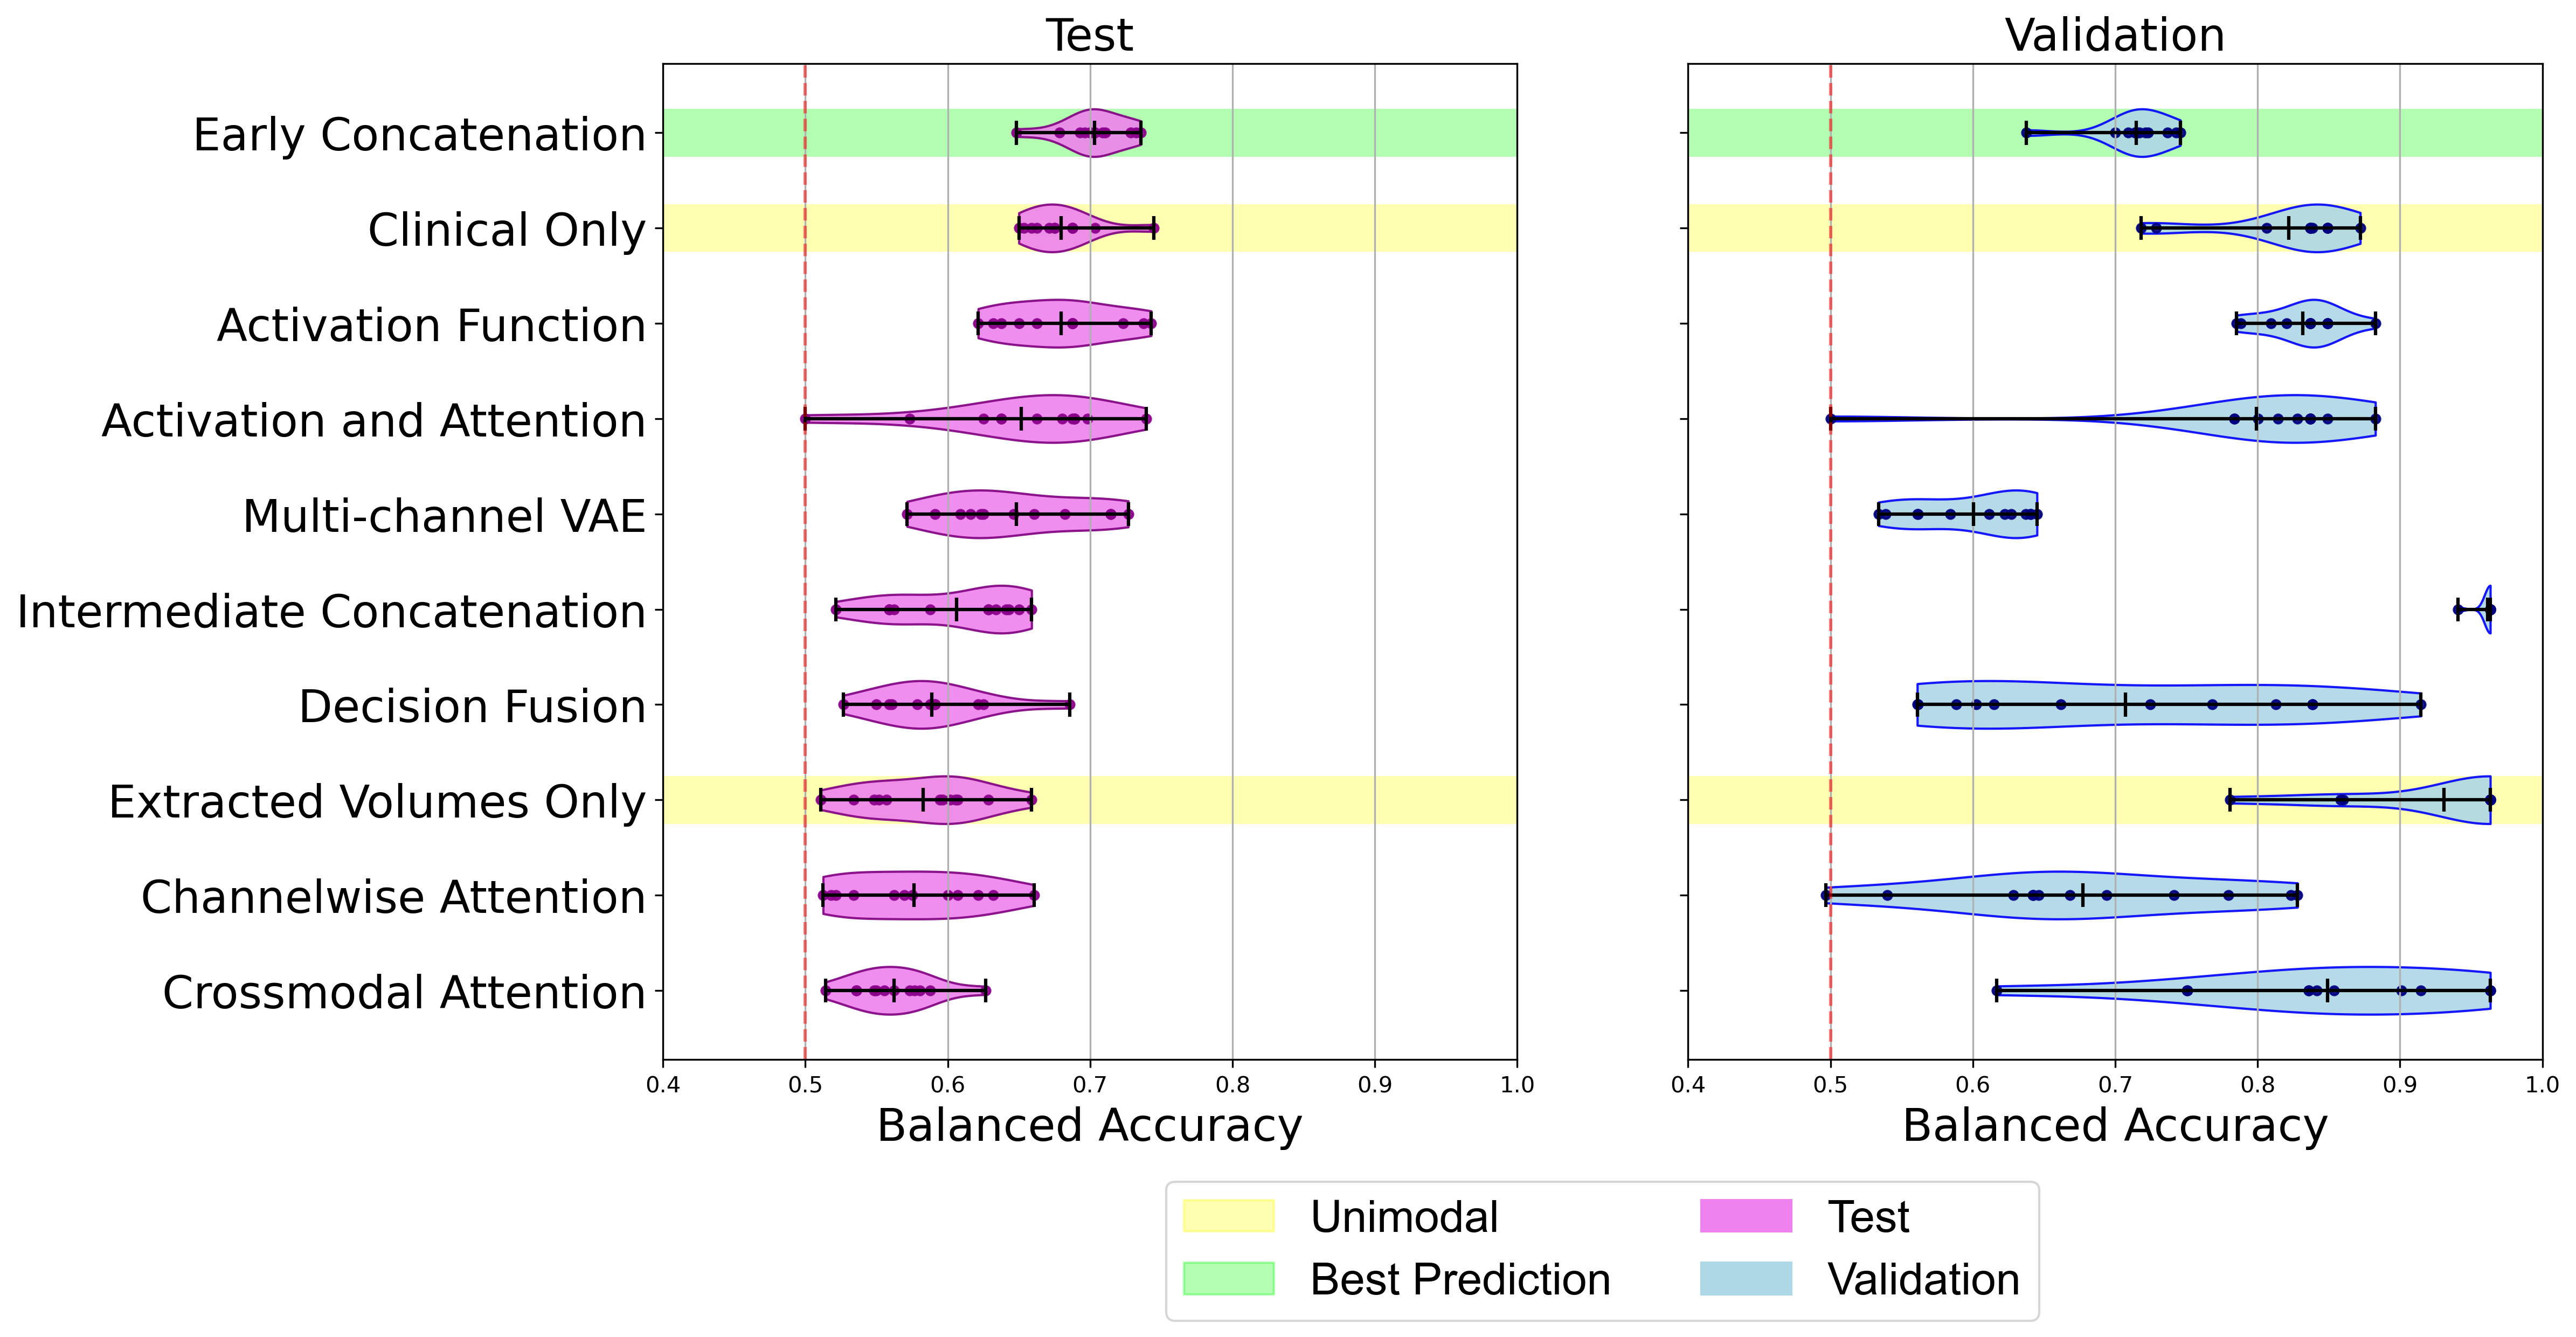
\includegraphics[width=1.2\linewidth]{figures/both_sites_together_balanced_accuracy_violin.png}
    \caption{Balanced accuracies of test set and validation set when sites trained together.}
    \label{fig:trainedtogetherviolin}
\end{figure}


\begin{table}[h]
\centering
\caption{Means and standard deviations of test metrics over repetitions of training on both sites. Bold is the best metric model.}
\label{tab:mnd_results}
\resizebox{\columnwidth}{!}{%
\begin{tabular}{lrrrrr} 

 & \multicolumn{5}{c}{\textbf{Performance metric: mean (standard deviation)}} \\
\textbf{Method} & Balanced Accuracy & AUROC & Precision & Recall & F1 \\ \hline
Clinical Only & 0.680 (0.025) & 0.748 (0.052) & \textbf{0.870 (0.044)} & 0.493 (0.049) & 0.627 (0.040) \\
Extracted Volumes Only & 0.583 (0.041) & 0.619 (0.038) & 0.695 (0.029) & 0.718 (0.101) & 0.703 (0.057) \\
Intermediate Concatenation & 0.606 (0.044) & 0.663 (0.029) & 0.708 (0.030) & \textbf{0.764 (0.036)} & \textbf{0.735 (0.029)} \\
Early Concatenation & \textbf{0.703 (0.023)} & \textbf{0.815 (0.014)} & 0.846 (0.018) & 0.598 (0.065) & 0.698 (0.044) \\
Channelwise Attention & 0.576 (0.047) & 0.596 (0.052) & 0.730 (0.059) & 0.486 (0.193) & 0.558 (0.137) \\
Crossmodal Attention & 0.562 (0.028) & 0.610 (0.041) & 0.681 (0.025) & 0.720 (0.079) & 0.697 (0.032) \\
Decision Fusion & 0.589 (0.040) & 0.647 (0.042) & 0.737 (0.030) & 0.488 (0.166) & 0.567 (0.141) \\
Multi-channel VAE & 0.648 (0.049) & 0.727 (0.048) & 0.833 (0.075) & 0.474 (0.084) & 0.597 (0.073) \\
Activation and Attention & 0.652 (0.061) & 0.712 (0.093) & 0.772 (0.237) & 0.451 (0.158) & 0.566 (0.186) \\
Activation Function & 0.680 (0.039) & 0.744 (0.054) & 0.868 (0.048) & 0.493 (0.620) & 0.626 (0.057) \\

\end{tabular}
}
\end{table}


\subsection{Training together}

Results from using all the training set together.

Table

\subsection{Train on one site, test on the other}

\begin{figure}
    \centering
    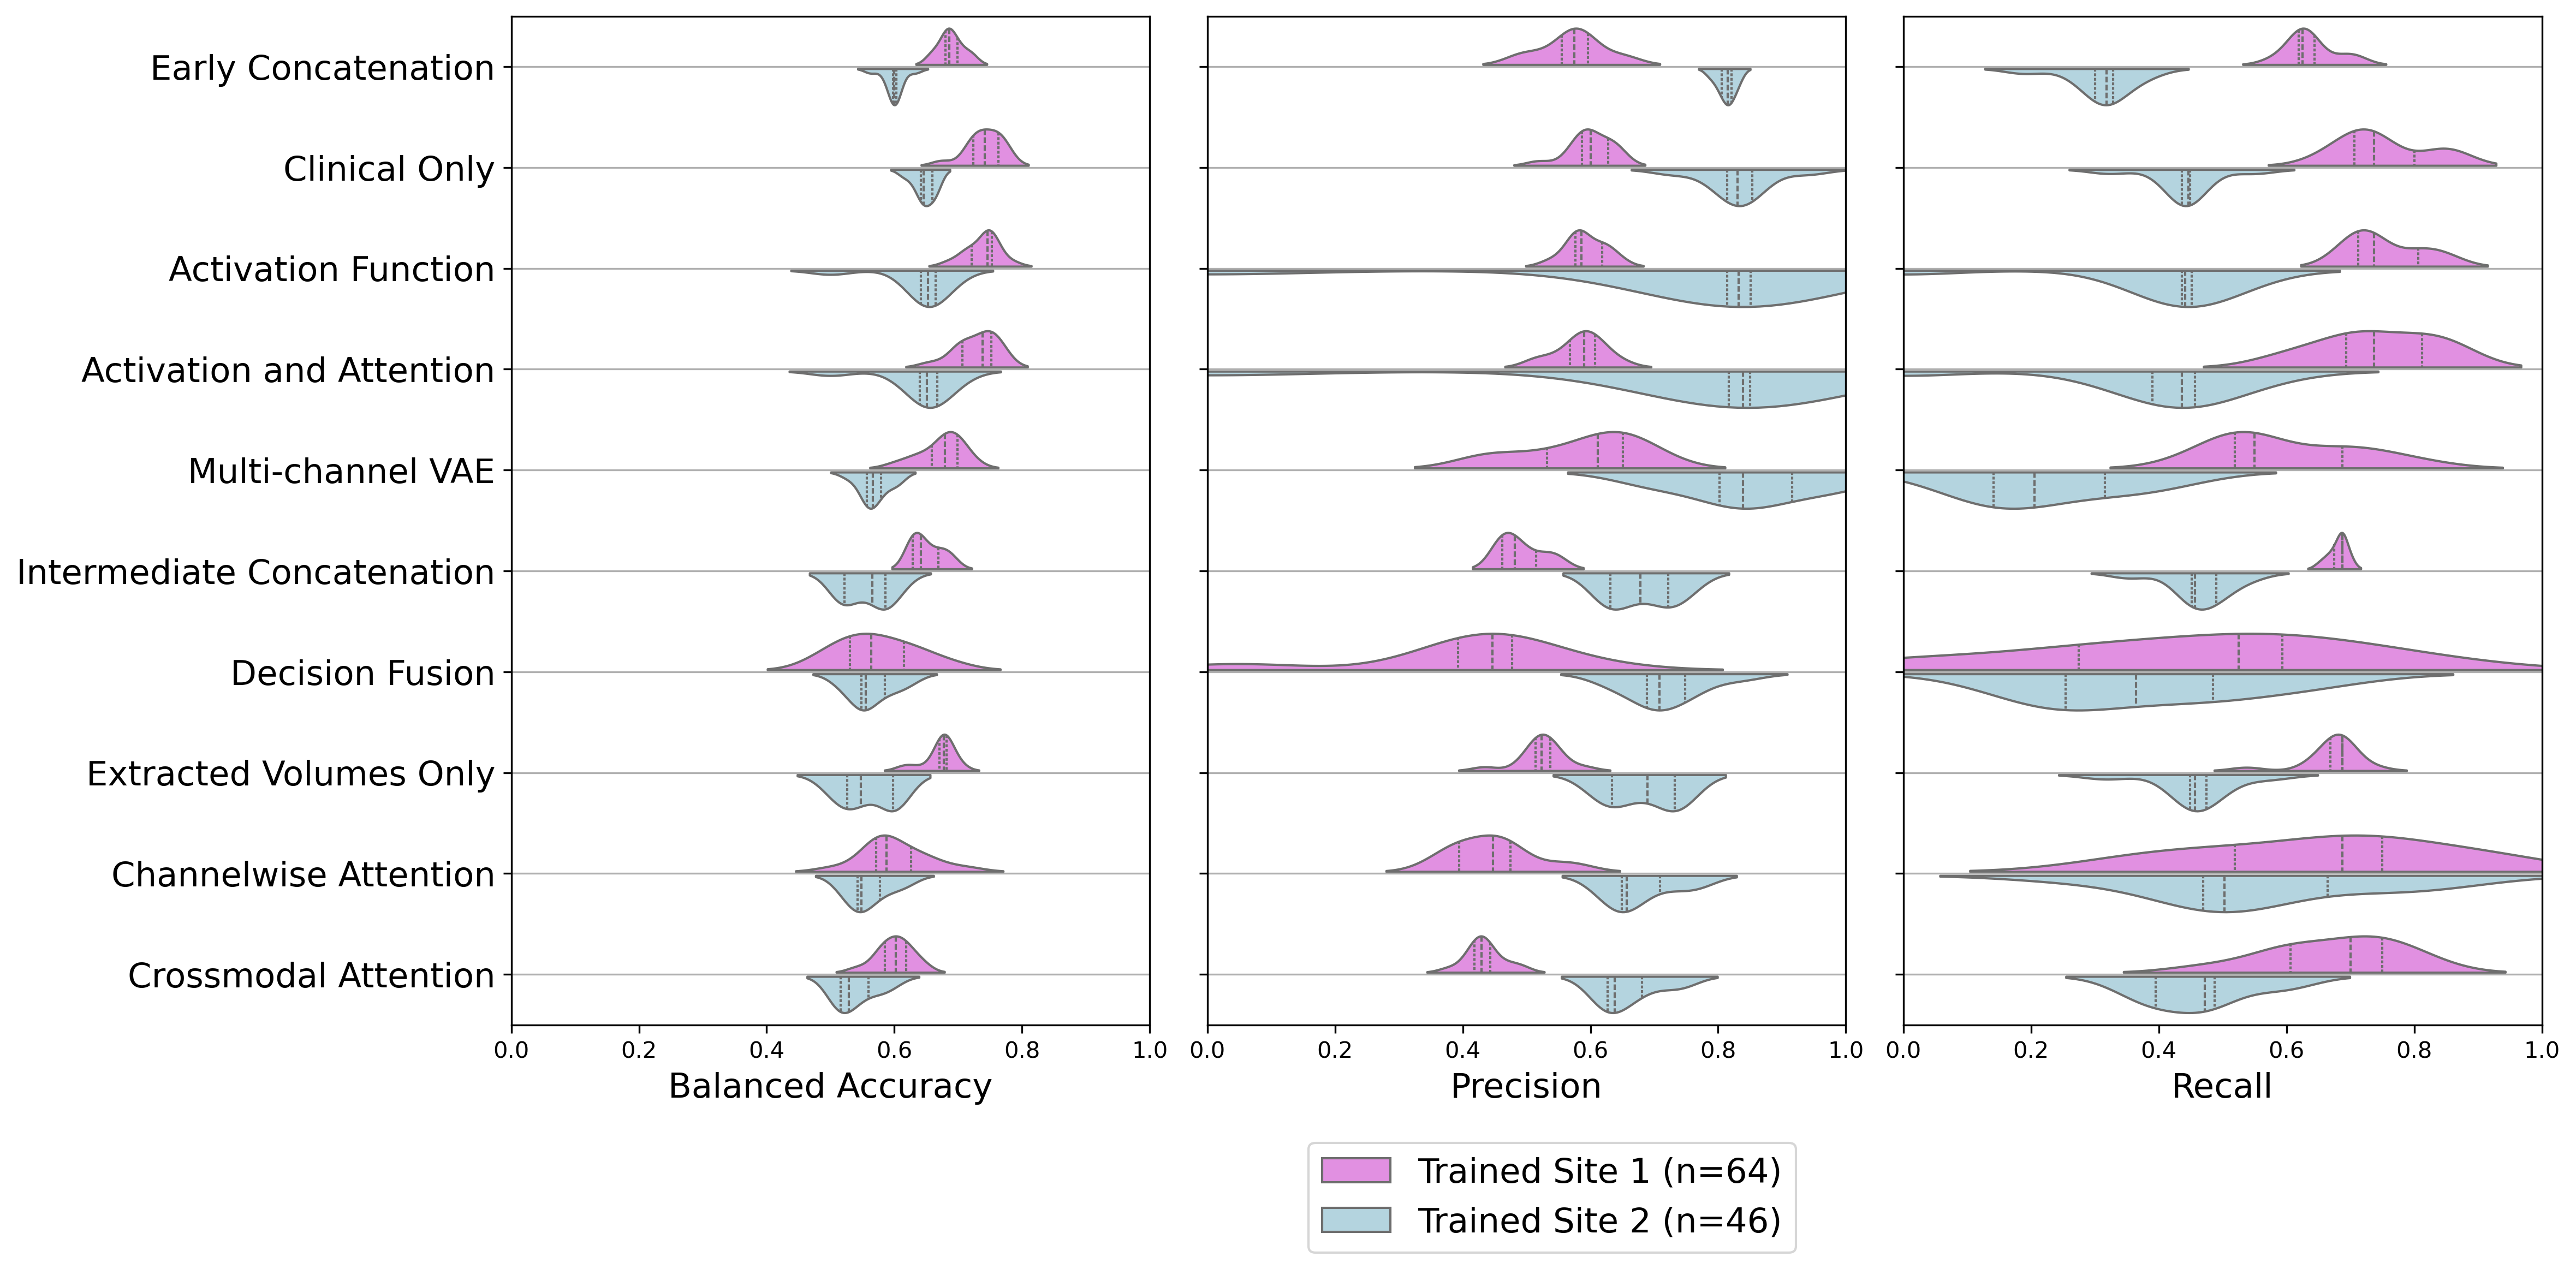
\includegraphics[width=0.8\textwidth]{figures/violinplot_site_effect}
    \caption{Effect of training on one site and testing on the other on the balanced accuracy of the different models. Ordered by best to worst model of trained together}
    \label{fig:site_effect}
\end{figure}

\textbf{Train on essex, test on milan}

Table

Figure

\textbf{Train on milan, test on essex}

Table

Figure

\section{Discussion}
\subsection{What does it mean??}
Interpreting the results.

\subsection{Limitations}
\begin{itemize}
    \item Limitations on sample size
    \item Evaluating on validation set rather than a completely external test set
    \item Predictive task of classification rather than regression: what if we used a regression task instead? Would that be more useful? It's a harder task so may require more data
    \item Limitation on using extracted brain volumes rather than raw MRI: what if the regions we've chosen aren't the most important ones? Subcortical regions have shown to have a role in MND, but we haven't included them here. *Look this up - the thalamus stuff*. However, whole image may introduce bias because further progressed patients may have worse quality scans.
    \item Two sites put together without harmonisation
    \item Using whole ALSFRS-R rather than individual components - not possible to get with Milan data
    \item Needs more hyperparameter tuning of the different models to see if they can be improved. Next steps would be to test different network architectures and hyperparameters to see if the results can be improved.
\end{itemize}

\section{Conclusion}
First look at multimodal data fusion in MND. What does it mean? What are the implications? What are the next steps?
\begin{itemize}
    \item If imaging + clinical is useful
    \begin{itemize}
        \item Let's add modalities
        \item Let's mix up the imaging preprocessing: DTI? Sub-cortical segmentation?
    \end{itemize}
    \item If imaging + clinical isn't useful
    \begin{itemize}
        \item Let's swap out the imaging for other modalities
        \item Let's try different machine learning models
        \item Let's mix up the imaging preprocessing: DTI? Sub-cortical segmentation?
    \end{itemize}
\end{itemize}
